%!TEX program = xelatex
\documentclass[dvipsnames, svgnames,a4paper,11pt]{article}
% ----------------------------------------------------
%   中山大学物理与天文学院本科实验报告模板
%   作者:Huanyu Shi,2019级
%   知乎:https://www.zhihu.com/people/za-ran-zhu-fu-liu-xing
%   Github:https://github.com/Huanyu-Shi/SYSU-SPA-Labreport-Template
%   Last update : 2023.4.10
% ----------------------------------------------------

% ----------------------------------------------------- 
%	加边框的命令
%	参考:https://tex.stackexchange.com/questions/531559/how-to-add-the-page-border-for-first-two-pages-in-latex
\usepackage{tikz}
\usetikzlibrary{calc}
\usepackage{eso-pic}
\AddToShipoutPictureBG{%
\begin{tikzpicture}[overlay,remember picture]
\draw[line width=0.6pt] % 边框粗细
    ($ (current page.north west) + (0.6cm,-0.6cm) $)
    rectangle
    ($ (current page.south east) + (-0.6cm,0.6cm) $); % 边框位置
\end{tikzpicture}}


\usepackage{xcolor}
\definecolor{c1}{HTML}{2752C9} % 目录颜色
\definecolor{c2}{RGB}{190,20,83} % 引用颜色

\usepackage{ctex}
\usepackage[top=28mm,bottom=28mm,left=15mm,right=15mm]{geometry}
\usepackage{hyperref} 
\hypersetup{
	colorlinks,
	linktoc = section, % 超链接位置,选项有section, page, all
	linkcolor = c1, % linkcolor 目录颜色
	citecolor = c1  % citecolor 引用颜色
}
\usepackage{amsmath,enumerate,multirow,float}
\usepackage{tabularx}
\usepackage{tabu}
\usepackage{subfig}
\usepackage{fancyhdr}
\usepackage{graphicx}
\usepackage{wrapfig}  
\usepackage{physics}
\usepackage{appendix}
\usepackage{amsfonts}

%
\usepackage{tcolorbox}
\tcbuselibrary{skins,breakable}
\newtcolorbox{tbox}[2][]{
    colframe=black!70!,
    breakable,
    enhanced,
	boxrule =0.5pt,
    title = {#2},
    fonttitle = \large\kaishu\bfseries,
	drop fuzzy shadow,
    #1
}
\newtcolorbox[auto counter,number within=section]{question}[1][]{
  top=2pt,bottom=2pt,arc=1mm,
  boxrule=0.5pt,
%   frame hidden,
  breakable,
  enhanced, %跨页后不会显示下边框
  coltitle=c1!80!gray,
  colframe=c1,
  colback=c1!3!white,
  drop fuzzy shadow,
  title={思考题~\thetcbcounter:\quad},
  fonttitle=\bfseries,
  attach title to upper,
  #1
}
\newcommand{\setLhead}[1]{%
  \lhead{{\color{gray}\kaishu #1}} % 定义新的命令,设置右边页眉的内容
}
\newcommand{\setRhead}[1]{%
  \rhead{{\color{gray}\kaishu #1}} % 定义新的命令,设置右边页眉的内容
}
% ---------------------------------------------------------------------
%	利用cleveref改变引用格式,\cref是引用命令
\usepackage{cleveref}
\crefformat{figure}{#2{\textcolor{c2}{图 #1}}#3} % 图片的引用格式
\crefformat{equation}{#2{(\textcolor{c2}{#1})}#3} % 公式的引用格式
\crefformat{table}{#2{\textcolor{c2}{表 #1}}#3} % 表格的引用格式


% ---------------------------------------------------------------------
%	页眉页脚设置
\fancypagestyle{plain}{\pagestyle{fancy}}
\pagestyle{fancy}
\setLhead{中山大学物理与天文学院基础物理实验预习报告}
%\lhead{\kaishu 中山大学物理与天文学院物理实验\uppercase\expandafter{\romannumeral3}} % 左边页眉,学院 + 课程
%\rhead{{\color{gray}\kaishu Template 实验报告模板}} % 右边页眉,实验报告标题
\setRhead{实验1\hspace{1pt}冰的熔化热测量}
\cfoot{\thepage} % 页脚,中间添加页码


% ---------------------------------------------------------------------
%	对目录、章节标题的设置
\renewcommand{\contentsname}{\centerline{\huge 目录}}
\usepackage{titlesec}
\usepackage{titletoc}
% \titleformat{章节}[形状]{格式}{标题序号}{序号与标题间距}{标题前命令}[标题后命令]
\titleformat{\section}{\centering\LARGE\songti}{}{1em}{}

% ---------------------------------------------------------------------
%   listing代码环境设置
\usepackage{listings}
\lstloadlanguages{python}
\lstdefinestyle{pythonstyle}{
backgroundcolor=\color{gray!5},
language=python,
frameround=tftt,
frame=shadowbox, 
keepspaces=true,
breaklines,
columns=spaceflexible,                   
basicstyle=\ttfamily\small, % 基本文本设置,字体为teletype,大小为scriptsize
keywordstyle=[1]\color{c1}\bfseries, 
keywordstyle=[2]\color{Red!70!black},   
stringstyle=\color{Purple},       
showstringspaces=false,
commentstyle=\ttfamily\scriptsize\color{green!40!black},%注释文本设置,字体为sf,大小为smaller
tabsize=2,
morekeywords={as},
morekeywords=[2]{np, plt, sp},
numbers=left, % 代码行数
numberstyle=\it\tiny\color{gray}, % 代码行数的数字字体设置
stepnumber=1,
rulesepcolor=\color{gray!30!white}
}




% ---------------------------------------------------------------------
%	其他设置
\def\degree{${}^{\circ}$} % 角度
\graphicspath{{./images/}} % 插入图片的相对路径
\allowdisplaybreaks[4]  %允许公式跨页 % 导入模板的相关设置
\usepackage{lipsum}
\usepackage{indentfirst}
\usepackage{pdfpages}
\usepackage{multirow}
\usepackage{subfig}
\usepackage{graphicx}
\usepackage{float} 
\usepackage{circuitikz}
\usepackage{diagbox}
\definecolor{mygreen}{rgb}{0,0.6,0}
\definecolor{mygray}{rgb}{0.5,0.5,0.5}
\definecolor{mymauve}{rgb}{0.58,0,0.82}
\lstset{
 backgroundcolor=\color{lightgray}, 
 basicstyle = \footnotesize,       
 breakatwhitespace = false,        
 breaklines = true,                 
 captionpos = b,                    
 commentstyle = \color{mygreen}\bfseries,
 extendedchars = false,             
 frame =shadowbox, 
 framerule=0.5pt,
 keepspaces=true,
 keywordstyle=\color{blue}\bfseries, % keyword style
 language = C++,                     % the language of code
 otherkeywords={string}, 
 numbers=left, 
 numbersep=5pt,
 numberstyle=\tiny\color{mygray},
 rulecolor=\color{black},         
 showspaces=false,  
 showstringspaces=false, 
 showtabs=false,    
 stepnumber=1,         
 stringstyle=\color{mymauve},        % string literal style
 tabsize=2,          
 title=\lstname                      
}
\renewcommand{\d}{\mathrm{d}}


%---------------------------------------------------------------------
%	正文
%---------------------------------------------------------------------
\setRhead{转动惯量测量和角动量守恒验证}%实验名称
\begin{document}


\begin{table}
	\renewcommand\arraystretch{1.7}
	\begin{tabularx}{\textwidth}{
		|X|X|X|X
		|X|X|X|X|}
	\hline
	\multicolumn{2}{|c|}{预习报告}&\multicolumn{2}{|c|}{实验记录}&\multicolumn{2}{|c|}{分析讨论}&\multicolumn{2}{|c|}{总成绩}\\
	\hline
	 25& &30  & &25  & &80& \\
	\hline
	\end{tabularx}
\end{table}


\begin{table}
	\renewcommand\arraystretch{1.7}
	\begin{tabularx}{\textwidth}{|X|X|X|X|}
	\hline
	专业:& 物理学类 &年级:& 2023级\\
	\hline
	姓名:& 姚昊廷  & 学号:&22322091\\
	\hline
	日期:& 2024.11.7& 教师签名:& \\
	\hline
	\end{tabularx}
\end{table}

\begin{center}
	\LARGE 转动惯量测量和角动量守恒验证
\end{center}

\textbf{【实验报告注意事项】}
\begin{enumerate}
	\item 实验报告由三部分组成:
	\begin{enumerate}
		\item 预习报告:(提前一周)认真研读\underline{\textbf{实验讲义}},弄清实验原理;实验所需的仪器设备、用具及其使用(强烈建议到实验室预习),完成课前预习思考题;了解实验需要测量的物理量,并根据要求提前准备实验记录表格(第一循环实验已由教师提供模板,可以打印)。预习成绩低于10分(共20分)者不能做实验。
	    \item 实验记录:认真、客观记录实验条件、实验过程中的现象以及数据。实验记录请用珠笔或者钢笔书写并签名(\textcolor{red}{\textbf{用铅笔记录的被认为无效}})。\textcolor{red}{\textbf{保持原始记录,包括写错删除部分,如因误记需要修改记录,必须按规范修改。}}(不得输入电脑打印,但可扫描手记后打印扫描件);离开前请实验教师检查记录并签名。
	    \item 分析讨论:\textcolor{red}{\textbf{处理实验原始数据(学习仪器使用类型的实验除外),结合误差理论的课程内容,对所有测量数据进行误差分析,转动惯量理论值、实验值、转动惯量变化前后的角动量测量值均用$A\pm \delta A$的形式表示,分析转动惯量理论值和实验值是否在误差范围内吻合,转动惯量变化前后的角动量测量值是否在误差范围内吻合;}}按规范呈现数据和结果(图、表),包括数据、图表按顺序编号及其引用;分析物理现象(含回答实验思考题,写出问题思考过程,必要时按规范引用数据);最后得出结论。
	\end{enumerate}
	\textbf{实验报告就是将预习报告、实验记录、和数据处理与分析合起来,加上本页封面。}
	\item 每次完成实验后的一周内交\textbf{实验报告}(特殊情况不能超过两周)。
	\item 除实验记录外,实验报告其他部分建议双面打印。
\end{enumerate}

{\textbf{【实验安全与实验室注意事项】}
\begin{enumerate}
	\item 实验前:要预习,明确实验目的和达成的目标;
	\item 实验中:取、放和安装待测物体时要轻拿轻放,不得摔碰;
	\item 不得随意拿取其它实验台的部件,如有缺失,请及时举手告知老师;
    \item 平台转动前,应注意保持转轴在垂直方向,即注意调节A型基座水平;
    \item 实验后:仔细分析处理数据,认真撰写实验报告。
    
\end{enumerate}}

\clearpage
\tableofcontents
\clearpage

\setcounter{section}{0}
\section{转动惯量测量和角动量守恒验证 \textbf{预习报告}}
	
\subsection{实验目的}
本实验的目的是通过实验测量出圆环和圆盘的转动惯量,并验证这些值与理论值计算值是否
一致。

\subsection{仪器用具}
\begin{table}[htbp]
	\centering
	\renewcommand\arraystretch{1.6}
	% \setlength{\tabcolsep}{10mm}
	\begin{tabular}{p{0.05\textwidth}|p{0.20\textwidth}|p{0.05\textwidth}|p{0.5\textwidth}}
	\hline
	编号& 仪器用具名称 & 数量 &  主要参数(型号,测量范围,测量精度等) \\
	\hline
	1&DataStudio程序&1 &\\
	\hline
	2&PASCO接口&1&\\
	\hline
	3&转动惯量组件& 1 &ME 8953 \\
	\hline
	4&摄影 /滑轮系统&1 &  \\
	\hline
	5&天平&1 &最小分度值0.01g  \\
	\hline
	6&卡钳&1 &最小分度值0.02mm \\
	\hline
	7&回形针&1 & \\
	\hline
	7&质量块和悬挂装置&1 & \\
	\hline
\end{tabular}
\end{table}

\textbf{【原理概述】}\\

理论上,围绕其质量中心转动的圆环的转动惯量$I$为:
$$I=\frac{1}{2}M(R_1^2+R_2^2)$$
其中$M$为圆环的质量,$R_1$为圆环的内径,$R_2$为圆环的外径。\\
圆盘绕其质心的转动惯量为
$$I=\frac{1}{2}MR^2$$
其中$M$为圆盘的质量,$R$为圆盘的半径。绕直径的转动惯量为
$$I=\frac{1}{4}MR^2$$
要通过实验找出转动惯量,需要对物体施加一个已知的扭矩,并测量由此产生的角加速度。
由于$\tau=I\alpha$
$$I=\tau\alpha$$
其中,$\alpha$是角加速度,等于$\frac{a}{r}$。$\tau$是重物悬挂在缠绕在仪器底座上的线上所产生的扭矩。
$$\tau=Tr$$
其中,$r$是缠绕线的圆柱体半径,$T$是设备旋转时线的张力。
对悬挂质量$m$应用牛顿第二定律,得出
$$\Sigma F=mg-T=ma$$
根据线的张力求解:$T=m(g-a)$

一旦确定了质量(m)的线加速度,就可以得到扭矩和角加速度,从而计算出转动惯量 。
\textbf{【实验前思考题】}
\begin{question}
	写出你认为实验中需要重点考虑的内容或注意事项
    \tcblower
    \begin{enumerate}
		\item 实验装置中的绕线柱应该尽可能调平。
		\item 实验三中待稳定后应迅速加上圆盘。
		\item 计算绕线半径时应考虑绳粗。
		\item 摩擦力平衡需准确。
	\end{enumerate}
\end{question}


\clearpage
\setLhead{中山大学物理与天文学院基础物理实验记录}
\begin{table}
	\renewcommand\arraystretch{1.7}
	\centering
	\begin{tabularx}{\textwidth}{|X|X|X|X|}
	\hline
	专业:& 物理学类 &年级:& 2023级 \\
	\hline
	姓名:& 姚昊廷 &学号:&22322091  \\
	\hline
	室温:&25.0$^\circ$C&实验地点:&A507\ F2\\
	\hline
	学生签名:& & 评分: &\\
	\hline
	实验时间:& 2024.11.7& 教师签名:&\\
	\hline
	\end{tabularx}
\end{table}

\section{转动惯量测量和角动量守恒验证 \textbf{实验记录}}
\textbf{【实验内容、步骤、结果】}(按照实验内容和步骤依次简要记录每项实验的“内容、步骤、结果”,注意包含实验数据、现象照片或现象描述等)\\
\begin{table}[htbp]
	\renewcommand\arraystretch{1.7}
	\centering
    \caption{实验1测量结果}
	\begin{tabularx}{\textwidth}{|l|X|X|X|X|X|l|}
	\hline
	\diagbox{测量对象}{测量次序}&1&2&3&4&5&结果(取置信概率99\%)\\
	\hline
	圆环质量(g)& 1433.43 &1433.46&1433.47&1433.47&1433.47&1433.46$\pm$0.03  \\
	\hline
	圆盘质量(g)& 1463.56&1463.59&1463.59&1463.59&1463.6&1463.59$\pm$0.03  \\
	\hline
	圆环内径(mm)&107.4&107.36&107.4&107.38&107.40&107.38$\pm$0.04\\
	\hline
	圆环外径(mm)&127.42&127.46&127.48&127.48&127.46&127.46$\pm$0.05\\
	\hline
	圆盘直径(cm)&22.85&22.85&22.90&22.90&22.90&22.88$\pm$0.06\\
	\hline
	\end{tabularx}
\end{table}
\begin{table}[H]
	\renewcommand\arraystretch{1.7}
	\centering
    \caption{转动惯量数据}
	\begin{tabularx}{\textwidth}{|X|X|X|}
	\hline
	&圆环与圆盘组合&单独圆盘\\
	\hline
	摩擦质量&12.5g &9.5g \\
	\hline
	悬挂质量&50g &50g \\
	\hline
	斜率&0.281293rad/s &0.49071rad/s \\
	\hline
	半径&8.77mm &8.77mm \\
	\hline
	\end{tabularx}
\end{table}
\begin{table}[H]
	\renewcommand\arraystretch{1.7}
	\centering
    \caption{结果}
	\begin{tabularx}{\textwidth}{|l|X|}
	\hline
	环盘整体的转动惯量&0.12912$\text{kg}\cdot\text{m}^2$(实验值),0.014488$\text{kg}\cdot\text{m}^2$(理论值)\\
	\hline
	圆盘的转动惯量(实验值)&0.8611$\text{kg}\cdot\text{m}^2$\\
	\hline
	圆环的转动惯量(实验值)&0.0053$\text{kg}\cdot\text{m}^2$\\
	\hline
	圆盘的转动惯量(理论值)&0.009119$\text{kg}\cdot\text{m}^2$\\
	\hline
	圆环的转动惯量(理论值)&0.005369$\text{kg}\cdot\text{m}^2$\\
	\hline
	圆盘竖直的转动惯量(实验值)&0.00488$\text{kg}\cdot\text{m}^2$\\
	\hline
	圆盘竖直的转动惯量(理论值)&0.004559$\text{kg}\cdot\text{m}^2$\\
	\hline
	圆盘转动惯量的百分比差异&-0.025\%\\
	\hline
	圆环转动惯量的百分比差异&-0.0034\%\\
	\hline
	圆盘竖直转动惯量的百分比差异&-0.0161\%\\
	\hline
	\end{tabularx}
\end{table}
验证角动量守恒:\\
圆盘的转动惯量(理论值):0.009119$\text{kg}\cdot\text{m}^2$\\
环盘整体的转动惯量(理论值):0.014488$\text{kg}\cdot\text{m}^2$\\
\begin{table}[H]
	\renewcommand\arraystretch{1.7}
	\centering
    \caption{验证角动量守恒结果}
	\begin{tabularx}{\textwidth}{|X|X|X|X|X|}
	\hline
	\multirow{2}{*}{角速度rad/s}&圆盘&3.749&5.686&6.377\\
	\cline{2-5}
	&环盘&2.394&3.581&3.906\\
	\hline
	\multirow{2}{*}{角动量$\text{kg}\cdot\text{m}^2\text{/s}$}&圆盘&0.034186&0.051849&0.05815\\
	\cline{2-5}
	&环盘&0.34684&.051881&0.056589\\
	\hline
	&百分比差异&1.4558\%&0.611\%&2.684\%\\
	\hline
	\end{tabularx}
\end{table}
\textcolor{red}{误差允许范围内可认为角动量守恒}
\subsection{实验过程中遇到的问题记录}



\clearpage
\setLhead{中山大学物理与天文学院基础物理实验分析与讨论}
\begin{table}
	\renewcommand\arraystretch{1.7}
	\begin{tabularx}{\textwidth}{|X|X|X|X|}
	\hline
	专业:& 物理学 &年级:& 2023级\\
	\hline
	姓名: &姚昊廷 & 学号:& 22322091\\
	\hline
    日期:&2024.11.7 & 评分: &\\
	\hline
	\end{tabularx}
\end{table}

\section{转动惯量测量和角动量守恒验证 分析与讨论}
\textbf{【分析与讨论】}(按照实验过程依次完成每项实验的“分析和讨论”)
\textcolor{red}{以圆盘绕中心轴的转动惯量误差计算为例。\textbf{分别给出圆盘绕中心轴的转动惯量、圆盘绕直径轴的转动惯量、圆筒的转动惯量、转动惯量变化前后的角动量结果的误差计算过程和分析结果。}}\\
\textbf{*随机误差合成方法:}
$$\sigma=\sqrt{\frac{\displaystyle\sum_{i=1}^{n} (l_i-\overline{l})^2}{n-1}}$$
\textbf{$n$为测量测量次数,$l_i$为单次测量值, $\overline{l}$为测量平均值}\\
\textbf{多次测量取平均值的随机误差计算方法:}\\
$$\sigma_y=\sqrt{(\frac{\partial f}{\partial x_1})^2\sigma_{x_1}^2+(\frac{\partial f}{\partial x_2})^2\sigma_{x_2}^2+\cdots+(\frac{\partial f}{\partial x_n})^2\sigma_{x_n}^2}$$
{\color{red}一、理论值
$$I_t=\frac{1}{2}MR^2$$
测量给出圆盘质量$M$,B类不确定度即天平精度取0.1g;测量给出圆盘半径$R$,B类不确定度若为游标卡尺测量精度取0.02mm,若为钢尺测量精度取0.2mm。通过误差传递计算,给出$I_t\pm \delta I_t$。

二、实验值
$$I_e=(m_c-m_f)r^2(\frac{g}{a}-1)$$
分别测量给出摩擦质量$m_f$和悬挂质量$m_t$,B类不确定度即天平精度取0.1g;测量给出圆柱半径$r$,B类不确定度即游标卡尺测量精度取0.02mm;重物下落加速度至少测量5次,分别给出各$a_i$的测量结果,统计给出其A类不确定度。通过误差传递计算,给出$I_e\pm \delta I_e$。

三、结果比较\\
利用计算数据比较法,判断测量结果是否存在系统误差。如满足下式,则两组结果间不存在系统误差。
$$|\overline{x}_i-\overline{x}_j|<2\sqrt{\sigma_i^2+\sigma_j^2}$$
}
一、(1)计算理论值
\begin{align*}
	I_1&=\frac{1}{2}MR^2=9.12\times10^{-3}\text{kg}\cdot\text{m}^2\text{(水平圆盘)}\\
	I_2&=\frac{1}{4}MR^2=4.56\times10^{-3}\text{kg}\cdot\text{m}^2\text{(竖直圆盘)}\\
	I_3&=\frac{1}{2}M(R_1^2+R_2^2)=5.36\times10^{-3}\text{kg}\cdot\text{m}^2\text{(水平圆环)}\\
\end{align*}
(2)B类不确度分析:游标卡尺:0.02mm,钢尺:0.2mm,天平0.1g。
\begin{align*}
	U_{r_1}&=\frac{0.02\text{mm}}{\sqrt{3}}=0.0115\text{mm}\\
	U_{r_2}&=\frac{0.2\text{mm}}{\sqrt{3}}=0.115\text{mm}\\
	U_{M}&=\frac{0.1\text{g}}{\sqrt{3}}=0.058\text{g}\\
\end{align*}
水平圆盘:
$$\delta I_1=\pm\sqrt{(\frac{\partial I_1}{\partial R}U_{r_2})^2+(\frac{\partial I_1}{\partial M}U_{M})^2}=\pm2.4\times10^{-6}\text{kg}\cdot\text{m}^2$$
竖直圆盘:
$$\delta I_2=\pm\sqrt{(\frac{\partial I_2}{\partial R}U_{r_2})^2+(\frac{\partial I_2}{\partial M}U_{M})^2}=\pm1.2\times10^{-6}\text{kg}\cdot\text{m}^2$$
圆环:
$$\delta I_3=\pm\sqrt{(\frac{\partial I_3}{\partial R_1}U_{r_1})^2+(\frac{\partial I_3}{\partial R_2}U_{r_2})^2+(\frac{\partial I_3}{\partial M}U_{M})^2}=\pm1.4\times10^{-6}\text{kg}\cdot\text{m}^2$$
(3)水平圆盘:$(9120\pm2.4)\times10^{-6}\text{kg}\cdot\text{m}^2$\\
竖直圆盘:$(4560\pm1.2)\times10^{-6}\text{kg}\cdot\text{m}^2$\\
圆环:$(5360\pm1.4)\times10^{-6}\text{kg}\cdot\text{m}^2$\\
二、实验值
(1)\begin{align*}
	I_1&=8.61\times10^{-3}\text{kg}\cdot\text{m}^2\\
	I_2&=4.88\times10^{-3}\text{kg}\cdot\text{m}^2\\
	I_3&=5.3\times10^{-3}\text{kg}\cdot\text{m}^2\\
\end{align*}
(2)A类不确定度:
\begin{align*}
	U_{a_1}&=\sqrt{\frac{\displaystyle\sum_{i=1}^3(I_1-\overline{I})^2}{3\times2}}=2.7\times10^{-4}\text{kg}\cdot\text{m}^2\\
	U_{a_2}&=\sqrt{\frac{\displaystyle\sum_{i=1}^3(I_2-\overline{I})^2}{3\times2}}=7.5\times10^{-4}\text{kg}\cdot\text{m}^2\\
	U_{a_3}&=\sqrt{\frac{\displaystyle\sum_{i=1}^3(I_3-\overline{I})^2}{3\times2}}=2.5\times10^{-5}\text{kg}\cdot\text{m}^2\\
\end{align*}
B类不确定度:
\begin{align*}
	U_{B_1}=\sqrt{(\frac{\partial I_1}{\partial R}U_{r_2})^2+(\frac{\partial I_1}{\partial M}U_{M})^2}=4.2\times10^{-5}\text{kg}\cdot\text{m}^2\\
	U_{B_2}=\sqrt{(\frac{\partial I_2}{\partial R}U_{r_2})^2+(\frac{\partial I_2}{\partial M}U_{M})^2}=2.6\times10^{-5}\text{kg}\cdot\text{m}^2\\
	U_{B_3}=\sqrt{(\frac{\partial I_3}{\partial R}U_{r_2})^2+(\frac{\partial I_3}{\partial M}U_{M})^2}=2.0\times10^{-5}\text{kg}\cdot\text{m}^2\\
\end{align*}
合成不确定度:
\begin{align*}
	U_{C_1}=\sqrt{U_{a_1}^2+U_{B_1}^2}=2.8\times10^{-5}\text{kg}\cdot\text{m}^2\\
	U_{C_2}=\sqrt{U_{a_2}^2+U_{B_2}^2}=7.9\times10^{-5}\text{kg}\cdot\text{m}^2\\
	U_{C_3}=\sqrt{U_{a_3}^2+U_{B_3}^2}=2.\times10^{-5}\text{kg}\cdot\text{m}^2\\
\end{align*}
水平圆盘:$I_1=(861\pm2.8)\times10^{-5}\text{kg}\cdot\text{m}^2$\\
竖直圆盘:$I_2=(488\pm7.9)\times10^{-5}\text{kg}\cdot\text{m}^2$\\
圆环:$I_3=(530\pm2.5)\times10^{-5}\text{kg}\cdot\text{m}^2$\\
三、结果比较
\begin{table}[H]
	\renewcommand\arraystretch{1.7}
	\centering
    \caption{比较}
	\begin{tabularx}{\textwidth}{|X|X|X|X|}
	\hline
	&水平圆盘&竖直圆盘&圆环\\
	\hline
	$|\overline{x}_i-\overline{x}_j|$&$5.08\times10^{-4}$&$3.2\times10^{-4}$&$6.9\times10^{-4}$\\
	\hline
	$2\sqrt{\sigma_i^2+\sigma_j^2}$&$1.01\times10^{-4}$&$1.58\times10^{-4}$&$5.09\times10^{-4}$\\
	\hline
	\end{tabularx}
\end{table}
三组均认为存在系统误差,可能原因有:
\begin{enumerate}
	\item 摩擦力平衡不准确;
	\item 测量工具存在系统误差。
\end{enumerate}
对于角动量守恒实验,则在误差允许范围内认为角动量守恒。
\clearpage
% ---------------------------------------------------------------------
%   参考文献
%   注:使用参考文献时应按照xelatex->bibtex->xelatex->xelatex顺序进行编译
\phantomsection
%\addcontentsline{toc}{section}{参考文献}
\bibliographystyle{unsrt}
\bibliography{myref}
%\begin{thebibliography}{9}
	%\bibitem{ref1} 凤飞龙,黄育红,金蔚,王公正,崔致远,“外推法计算冰的熔解热的理论依据及Matlab实现方案”,《大学物理》,第42卷,第2期
%\end{thebibliography}


\clearpage
\appendix
\appendixpage
\addappheadtotoc


%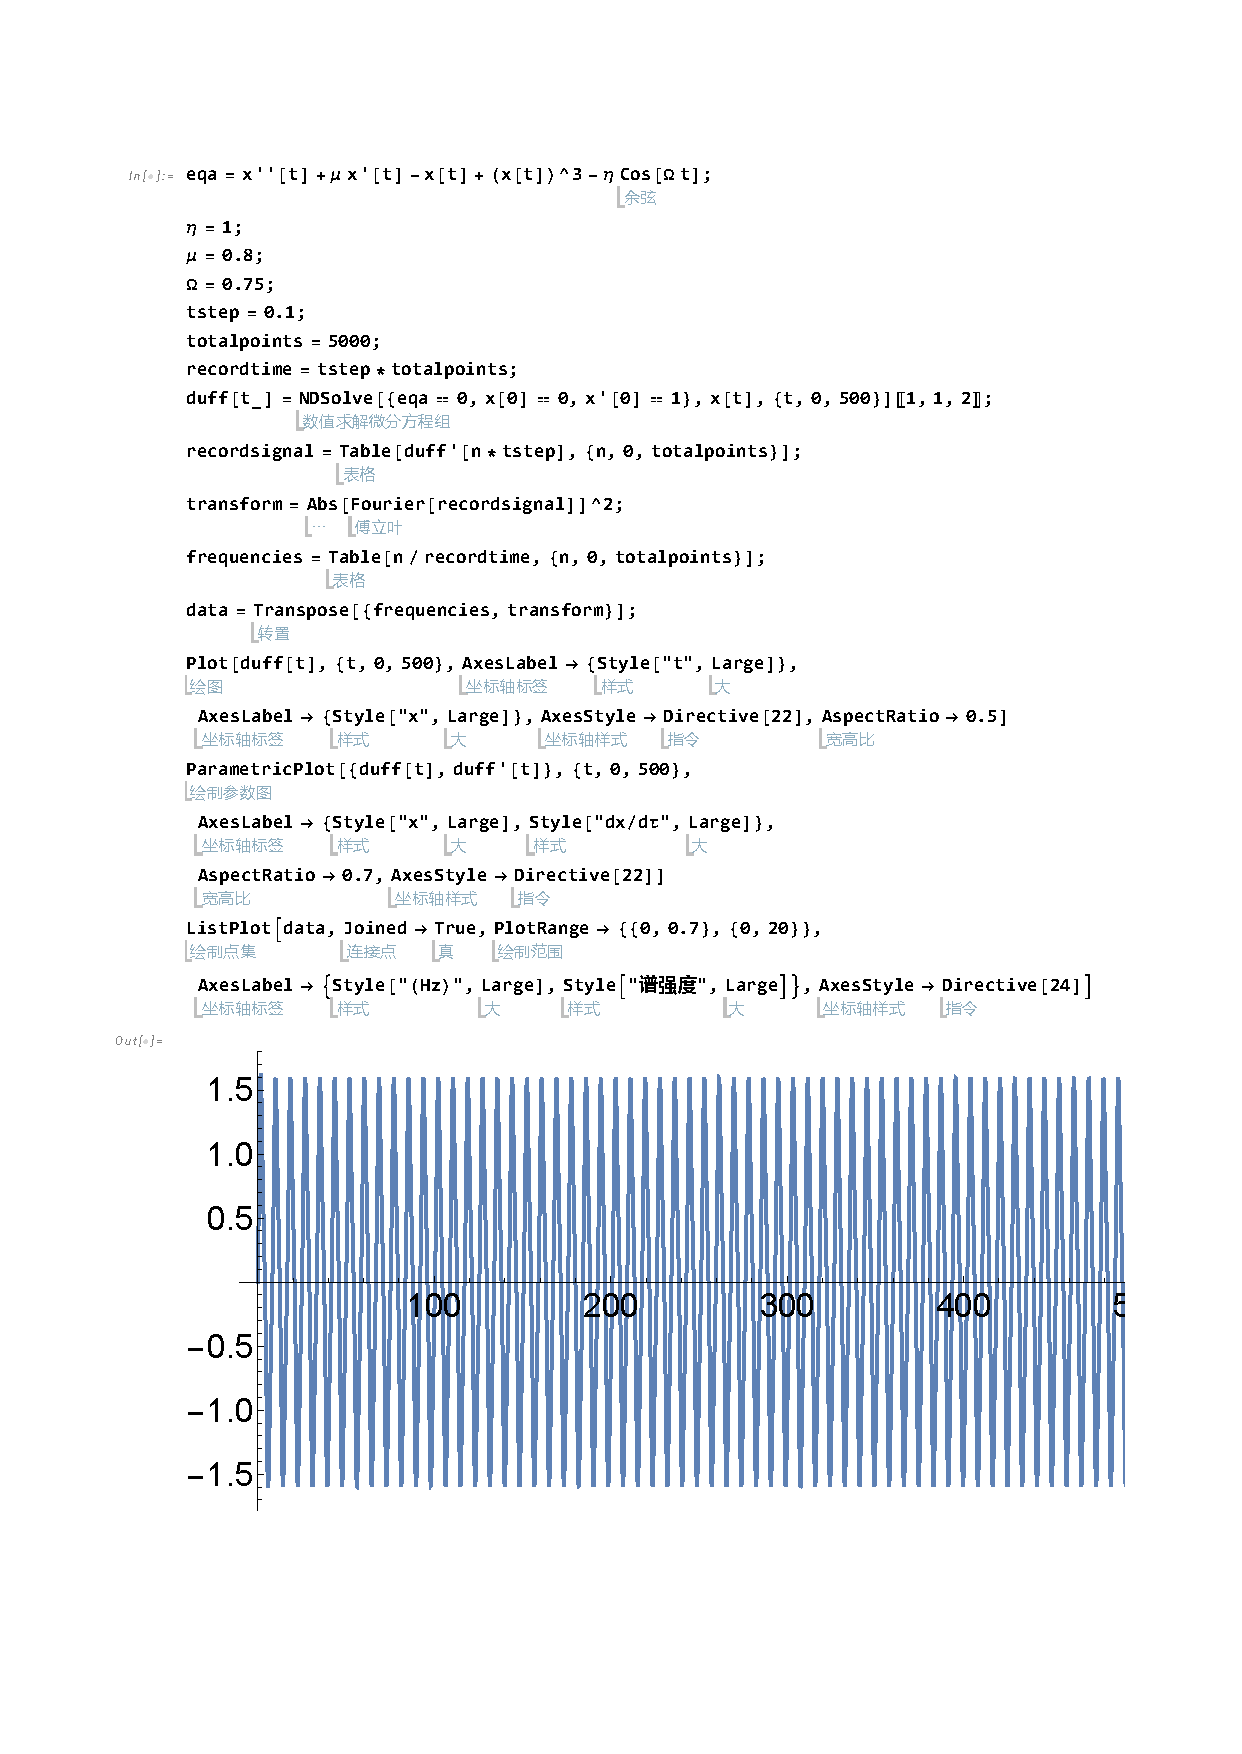
\includepdf[pages=-]{chaos.pdf}
\subsection*{原件扫描}
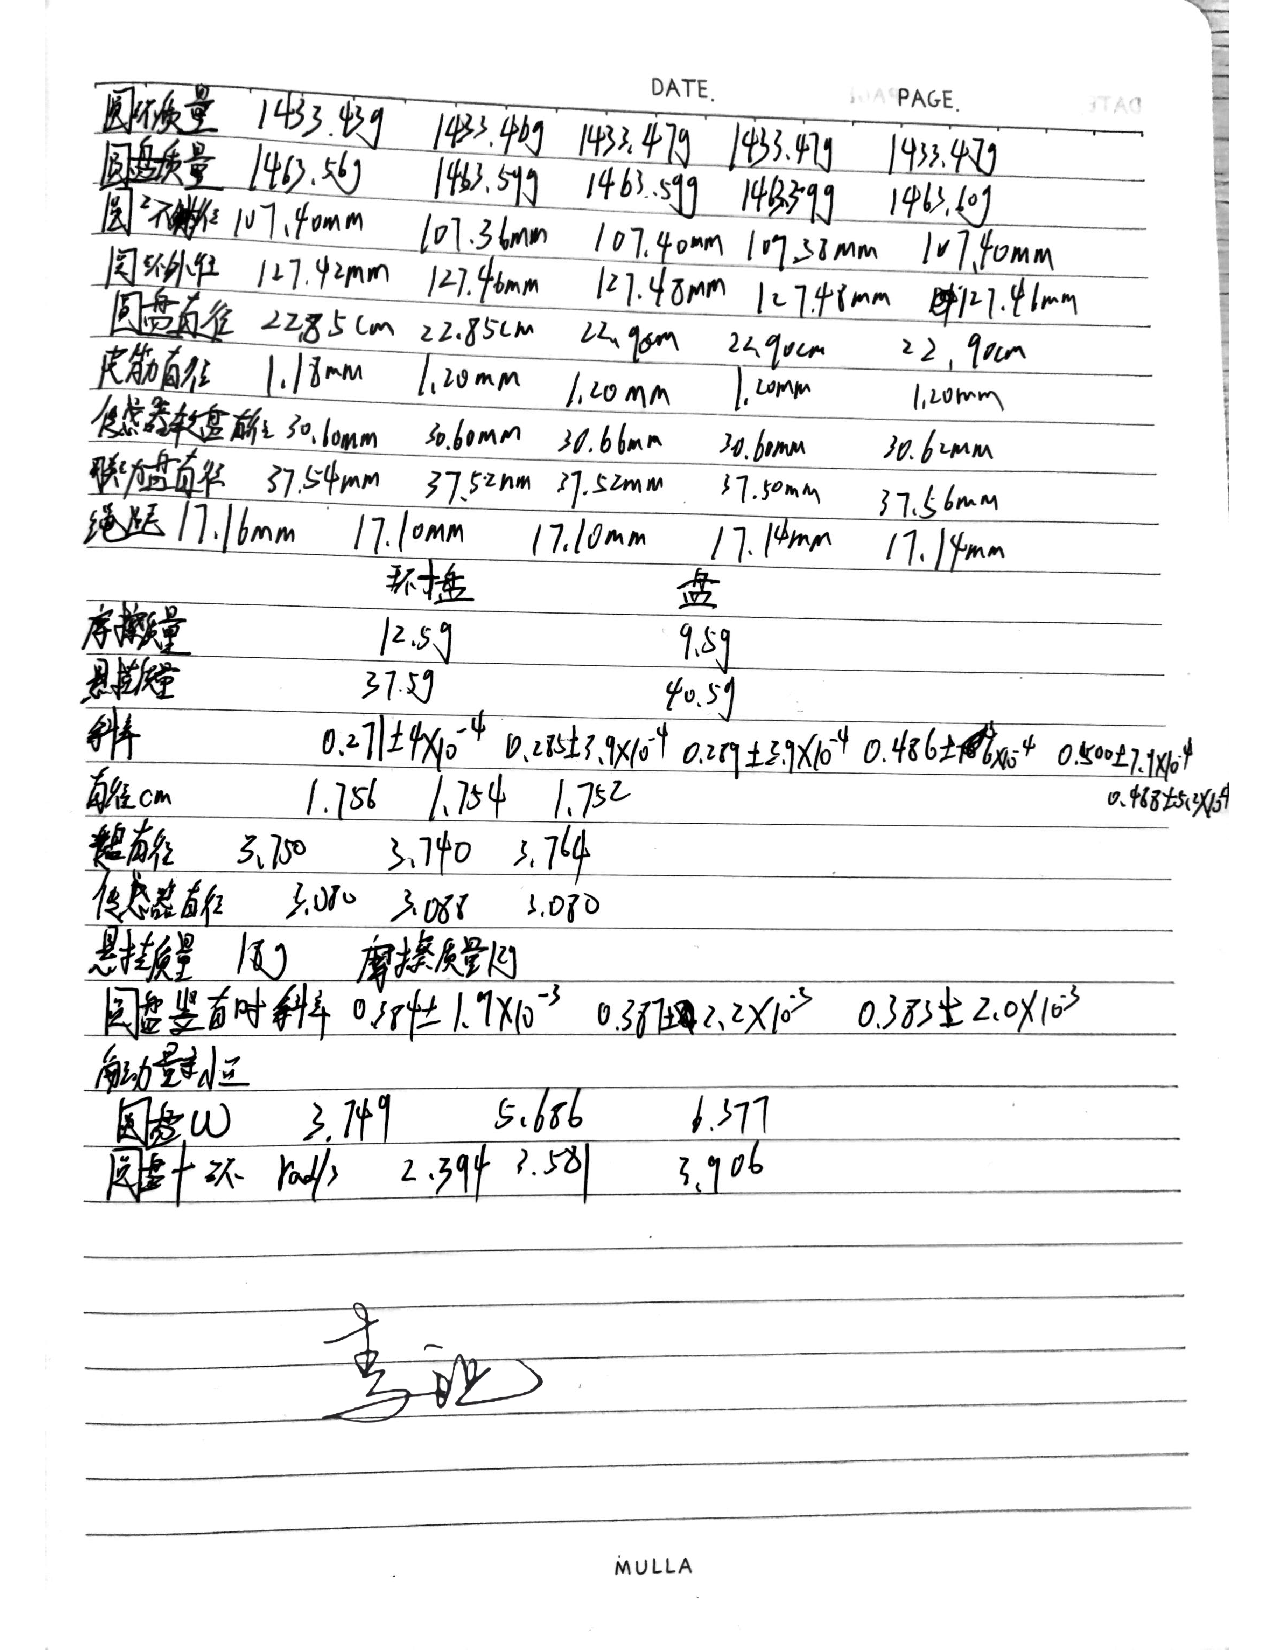
\includepdf[pages=-]{实验6原件.pdf}

\subsection*{桌面}
\begin{figure}[!h]
	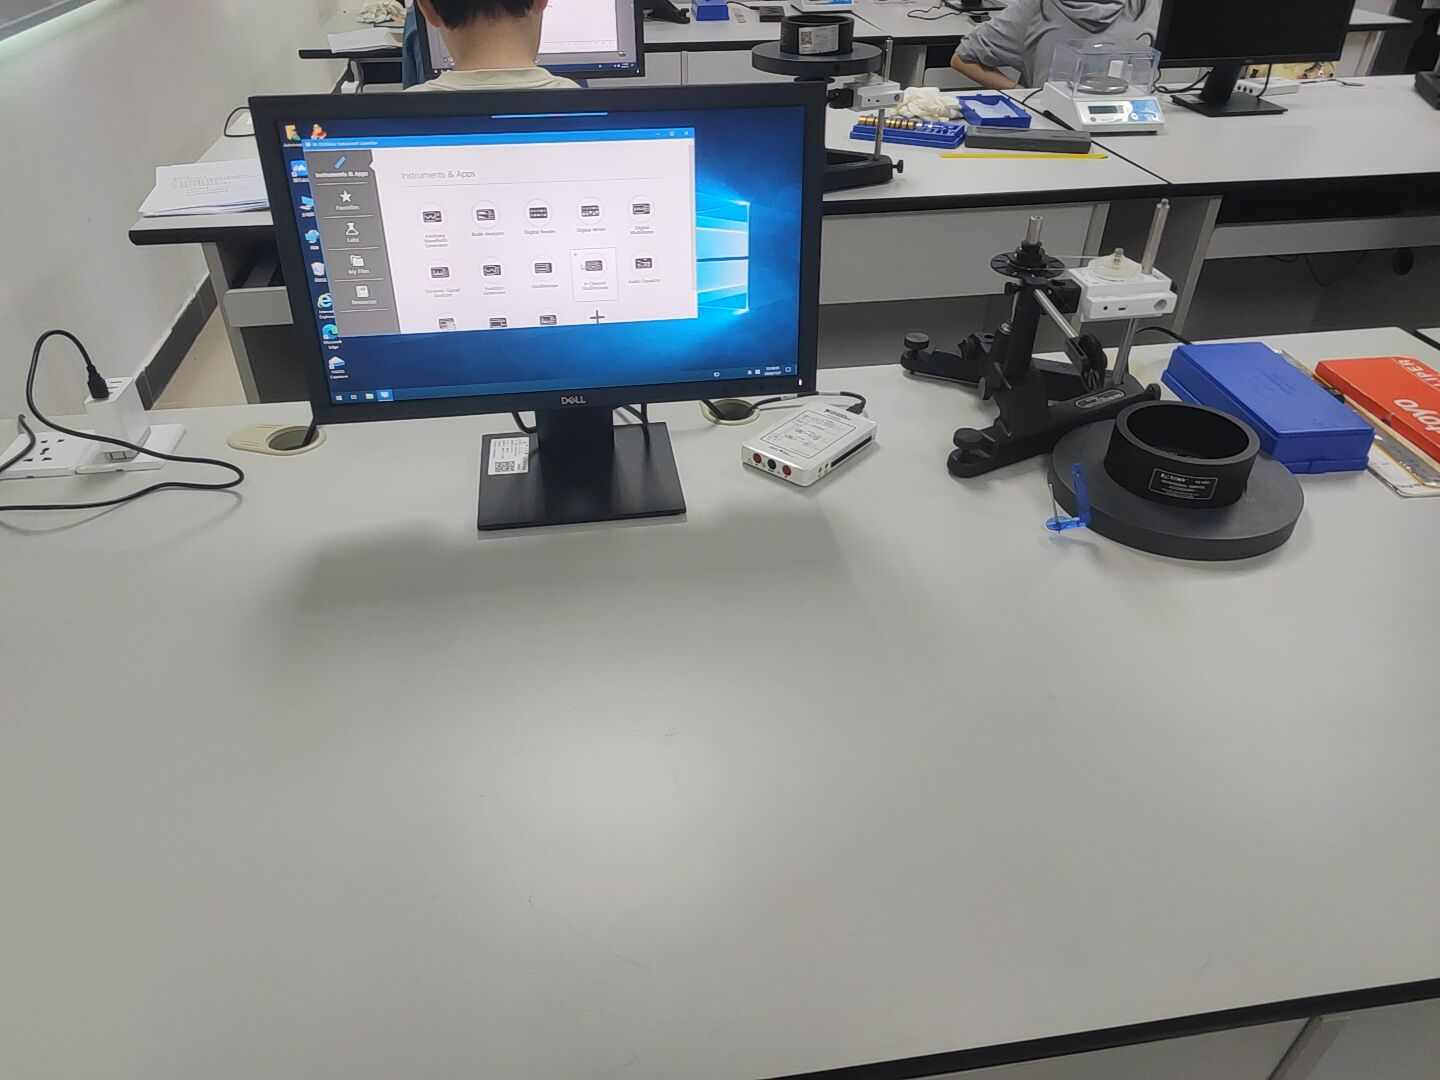
\includegraphics[width=0.95\textwidth]{实验6桌面.jpg}
\end{figure}
\end{document} 